\noindent

\includegraphics[height=1.25cm]{images/pictograms/benchmark}

\includegraphics[height=1.25cm]{images/pictograms/FDM}

\includegraphics[height=1.25cm]{images/pictograms/temperature}

%%%%%%%%%%%%%%%%%%%%%%%%%%%%%%%%%%%%%%%%%%%%%%%%%%%%%%%%%%%%%%%%%%%%%%%%%%%%%%%%%%%%%%%%%%%%%%%%%%%

\begin{flushright} {\tiny {\color{gray} python\_codes/fieldstone\_180/text.tex}} \end{flushright}

%\lstinputlisting[language=bash,basicstyle=\small]{python_codes/template_keywords.key}

\par\noindent\rule{\textwidth}{0.4pt}

\begin{center}
\inpython
{\small Code: \url{https://github.com/cedrict/fieldstone/tree/master/python_codes/fieldstone_180}}
\end{center}

\par\noindent\rule{\textwidth}{0.4pt}

{\sl This stone was developed with input from H. Brett}. \index{contributors}{H. Brett}

\par\noindent\rule{\textwidth}{0.4pt}

Last revision: September 5th, 2025.

\par\noindent\rule{\textwidth}{0.4pt}

%%%%%%%%%%%%%%%%%%%%%%%%%%%%%%%%%%%%%%%%%%%%%%%%%%%%%%%%%%%%%%%%%%%%%%%%%%%%%%%%%%%%%%%%%%%%%%%%%%%

Let us consider the following 1d mesh composed of four nodes:
\begin{center}
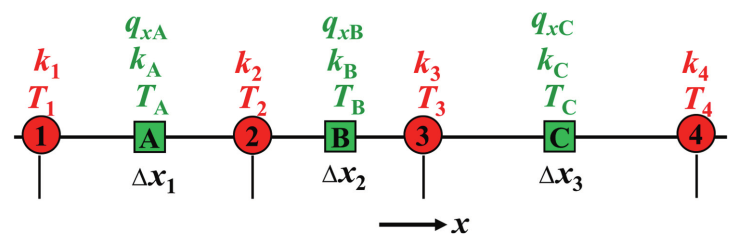
\includegraphics[width=10cm]{python_codes/fieldstone_180/gerya_stencil}\\
{\captionfont I need to redo the figure and replace $\Delta x_i$ by $h_i$.}
\end{center}
We denote by A,B,C the positions of the middle of each cell.
We assume for simplicity that we prescribe temperature 
boundary conditions on nodes 1 and 4.
We wish to solve the steady state diffusion equation $\vec\nabla \cdot (-k \vec\nabla T)=0$
in the case where the heat conductivity is not necessarily constant in space.

Following Section 10.2 of \textcite{gery19book}, we follow the
proposer conservative Finite Difference formulation of the flux terms
and we write the heat flux at nodes 2 and 3 as follows:
\begin{eqnarray}
\left.\frac{dq}{dx}\right|_2 &=& \frac{q_B-q_A}{(h_1+h_2)/2} \nn\\
\left.\frac{dq}{dx}\right|_3 &=& \frac{q_C-q_B}{(h_2+h_3)/2} \nn
\end{eqnarray}

We choose\footnote{Note that in the book Gerya presents 
another way of averaging the conductivity, i.e. a harmonic averaging.} 
\[
k_A = \frac{k_1+k_2}{2}
\qquad
k_B = \frac{k_2+k_3}{2}
\qquad
k_C = \frac{k_3+k_4}{2}
\]
so that we have for instance
\begin{eqnarray}
\left.\frac{dq}{dx}\right|_3
&=& \frac{q_C-q_B}{(h_2+h_3)/2} \nn\\
&=& \frac{-k_C \frac{T_4-T_3}{h_3} + k_B \frac{T_3-T_2}{h_2}  }{(h_2+h_3)/2} \nn\\
&=& \frac{- \frac{k_3+k_4}{2} \frac{T_4-T_3}{h_3} + \frac{k_2+k_3}{2} \frac{T_3-T_2}{h_2}  }{(h_2+h_3)/2} \nn\\
&=& -\frac{k_3+k_4}{h_3(h_2+h_3)} (T_4-T_3)+  \frac{k_2+k_3}{h_2(h_2+h_3)} (T_3-T_2)\nn
\end{eqnarray}
and finally
\[
\left.\frac{dq}{dx}\right|_3
=
-\frac{k_2+k_3}{h_2(h_2+h_3)} T_2
+ \left(
\frac{k_3+k_4}{h_3(h_2+h_3)} + \frac{k_2+k_3}{h_2(h_2+h_3)} 
\right) T_3
-\frac{k_3+k_4}{h_3(h_2+h_3)} T_4
\]
This leads in the end to the following stencil for the inside nodes:
\[
\frac{dq}{dx}|_i
= - \frac{k_{i-1}+k_i}{h_{i-1} (h_{i-1}+h_i)} T_{i-1}
+\left(
\frac{k_{i}+k_{i+1}}{h_{i} (h_{i-1}+h_i)} +
\frac{k_{i-1}+k_i}{h_{i-1} (h_{i-1}+h_i)}
\right) T_i
 - \frac{k_{i}+k_{i+1}}{h_{i} (h_{i-1}+h_i)} T_{i+1}
\]
Note that stencil does not lead to symmetric matrix, even for a diffusion equation!

Of course it is trivial to verify that if the node spacing is constant and the 
heat conductivity is also constant then the stencil above simply becomes 
\[
\frac{dq}{dx}|_i = -k \frac{T_{i-1}-2T_i+T_{i+1}}{h^2}
\] 

%%%%%%%%%%%%%%%%%%%%%%%%%%%%%%%%%%%%%%%%%%%%%%%%%%%%%%%%%%%%%%
\section*{A simple example}

Let us consider the case of 5 nodes inside the segment $[0,1]$:
\begin{lstlisting}
nnx=5                         
x=np.array([0,0.3,0.4,0.9,1]) 
\end{lstlisting}
We set $k=1$ for all nodes:
\begin{lstlisting}
hcond=np.ones(nnx)  
\end{lstlisting}
The cell sizes are then computed as follows\footnote{There is surely a more python
way of doing this}:
\begin{lstlisting}
h=np.zeros(nnx-1,dtype=np.float64)
for i in range(0,nnx-1):
    h[i]=x[i+1]-x[i]
\end{lstlisting}
The matrix and rhs of the linear system are declared:
\begin{lstlisting}
b=np.zeros(nnx,dtype=np.float64)
A=lil_matrix((nnx,nnx),dtype=np.float64)
\end{lstlisting}
Boundary conditions are then applied, in this case $T_0=0$ and $T_4=1$, 
which translates as follows:
\begin{lstlisting}
A[0,0]=1         ; b[0]=0     # left boundary condition
A[nnx-1,nnx-1]=1 ; b[nnx-1]=1 # right boundary condition
\end{lstlisting}
For each internal node the stencil is applied:
\begin{lstlisting}
for i in range(1,nnx-1):
    A[i,i-1]=-(hcond[i-1]+hcond[i])/h[i-1]/(h[i-1]+h[i])
    A[i,i]  = (hcond[i+1]+hcond[i])/h[i]  /(h[i-1]+h[i]) \
            + (hcond[i-1]+hcond[i])/h[i-1]/(h[i-1]+h[i]) 
    A[i,i+1]=-(hcond[i+1]+hcond[i])/h[i]  /(h[i-1]+h[i]) 
\end{lstlisting}
Finally the linear system is solved and the temperature 
field is obtained:
\begin{lstlisting}
T=sps.linalg.spsolve(sps.csr_matrix(A),b)
\end{lstlisting}
When printing the temperature solution we find 
\begin{lstlisting}
T= [0.  0.3 0.4 0.9 1. ] 
\end{lstlisting}
which is a straight line between 0 and 1, as expected.





